\chapter{Астронавигационные таблицы и номограммы}\label{app:4}

\section*{A. Навигационные звёзды}

{\centering
  \footnotesize
  \begin{tabular}{r|l|l|c|c|c|c|c}
    \toprule
      & \shortstack{Собственное \\ имя }
                 & \shortstack{Обозначение \\ в созвездии }
                 & \shortstack{Блеск \\ $m$}
                 & \shortstack{Склонение \\ $\delta$}
                 & \shortstack{Звёздный \\ угол \\ \taustar}
                 & \shortstack{Годовое \\ $\Delta \delta$}
                 & \shortstack{Годовое \\ $\Delta \taustar$} \\
    \midrule
    1 & Дубхе    & \alphaStar{Большой медведицы}
                 & $+2,0$ & \grmmr{61}{51,7}{N} & \grmm{194}{22,7} & $-0,32'$ & $-0,92'$ \\
    2 & Фекда    & \gammaStar{Большой Медведицы}
                 & $+2,5$ & \grmmr{53}{48,5}{N} & \grmm{181}{48,3} & $-0,33'$ & $-0,78'$ \\
    3 & Бенетнаш & \etaStar{Большой Медведицы}
                 & $+1,9$ & \grmmr{49}{25,0}{N} & \grmm{153}{18,5} & $-0,30'$ & $-0,59'$ \\
    4 & Полярная & \alphaStar{Малой Медведицы}
                 & $+2,1$ & \grmmr{89}{10,1}{N} & \grmm{327}{02,0} & $+0,27'$ & $-11,68'$ \\
    5 & Регул    & \alphaStar{Льва}
                 & $+1,3$ & \grmmr{12}{03,9}{N} & \grmm{208}{10,4} & $-0,29'$ & $-0,80'$ \\
    6 & Арктур   & \alphaStar{Волопаса}
                 & $+0,2$ & \grmmr{19}{17,3}{N} & \grmm{146}{18,5} & $-0,31'$ & $-0,68'$ \\
    7 & Спика    & \alphaStar{Девы}
                 & $+1,2$ & \grmmr{11}{03,5}{S} & \grmm{158}{57,5} & $+0,31'$ & $-0,79'$ \\
    8 & Вега     & \alphaStar{Лиры}
                 & $+0,1$ & \grmmr{38}{46,0}{N} & \grmm{\ 80}{55,5}& $+0,06'$ & $-0,51'$ \\
    9 & Денеб    & \alphaStar{Лебедя}
                 & $+1,3$ & \grmmr{45}{12,6}{N} & \grmm{\ 49}{48,6}& $+0,22'$ & $-0,51'$ \\
    10 & Альтаир & \alphaStar{Орла}
                 & $+0,9$ & \grmmr{\ 8}{49,0}{N}& \grmm{\ 62}{32,4}& $+0,15'$ & $-0,73'$ \\
    11 & Антарес & \alphaStar{Скорпиона}
                 & $+1,2$ & \grmmr{26}{23,3}{S} & \grmm{112}{56,7} & $+0,13'$ & $-0,92'$ \\
    12 & Кафф    & \betaStar{Кассиопеи}
                 & $+2,4$ & \grmmr{59}{02,2}{N} & \grmm{357}{57,9} & $+0,33'$ & $-0,80'$ \\
    13 & Альферас & \alphaStar{Андромеды}
                 & $+2,2$ & \grmmr{28}{58,8}{N} & \grmm{358}{09,4} & $+0,33'$ & $-0,78'$ \\
    14 & Мирфак  & \alphaStar{Персея}
                 & $+1,9$ & \grmmr{49}{47,3}{N} & \grmm{309}{16,6} & $+0,21'$ & $-1,07'$ \\
    15 & Капелла & \alphaStar{Возничего}
                 & $+0,2$ & \grmmr{45}{58,6}{N} & \grmm{281}{12,0} & $+0,06'$ & $-1,11'$ \\
    16 & Бетельгейзе & \alphaStar{Ориона}
                 & $+0,1$ & \grmmr{\ 7}{24,2}{N}& \grmm{271}{28,8} & $+0,01'$ & $-0,81'$ \\
    17 & Альдебаран & \alphaStar{Тельца}
                 & $+1,1$ & \grmmr{16}{28,1}{N} & \grmm{291}{18,5} & $+0,12'$ & $-0,86'$ \\
    18 & Сириус  & \alphaStar{Большого Пса}
                 & $-1,6$ & \grmmr{16}{41,4}{S} & \grmm{258}{56,2} & $+0,08'$ & $-0,66'$ \\
    19 & Поллукс & \betaStar{Близнецов}
                 & $+1,2$ & \grmmr{28}{04,4}{N} & \grmm{243}{58,7} & $-0,15'$ & $-0,92'$ \\
    20 & Процион & \alphaStar{Малого Пса}
                 & $+0,5$ & \grmmr{\ 5}{16,5}{N}& \grmm{245}{26,3} & $-0,16'$ & $-0,78'$ \\
    \bottomrule
  \end{tabular}
}

\textbf{Примечания:}
\begin{enumerate}
\item Координаты звёзд даны на лето 1980~г. В другие сезоны они могут
  отличаться до $0,5'$.
\item В последующие годы координаты звёзд получаются добавлением
  величин годовых их изменений, умноженных на число лет, прошедших
  после 1980~г.
\end{enumerate}

\clearpage
\section*{Б. Перевод дуговой меры во временн\'{у}ю и обратно}

\begin{center}
  
  \textbf{Градусы}

  {\scriptsize
    \begin{tabularx}{\linewidth}{c|X|X|X|X|X|X|X|X|X|X|c}
      \toprule
      \gr & 0\gr & 1\gr & 2\gr & 3\gr & 4\gr & 5\gr & 6\gr & 7\gr & 8\gr & 9\gr & \gr \\
      \midrule
      0\gr & \hhmm{00}{00} & \hhmm{00}{04} & \hhmm{00}{08} & \hhmm{00}{12} & \hhmm{00}{16} & \hhmm{00}{20} & \hhmm{00}{24} & \hhmm{00}{28} & \hhmm{00}{32} & \hhmm{00}{36} & 0\gr \\ 
      10\gr & \hhmm{00}{40} & \hhmm{00}{44} & \hhmm{00}{48} & \hhmm{00}{52} & \hhmm{00}{56} & \hhmm{01}{00} & \hhmm{01}{04} & \hhmm{01}{08} & \hhmm{01}{12} & \hhmm{01}{16} & 10\gr \\ 
      20\gr & \hhmm{01}{20} & \hhmm{01}{24} & \hhmm{01}{28} & \hhmm{01}{32} & \hhmm{01}{36} & \hhmm{01}{40} & \hhmm{01}{44} & \hhmm{01}{48} & \hhmm{01}{52} & \hhmm{01}{56} & 20\gr \\ 
      30\gr & \hhmm{02}{00} & \hhmm{02}{04} & \hhmm{02}{08} & \hhmm{02}{12} & \hhmm{02}{16} & \hhmm{02}{20} & \hhmm{02}{24} & \hhmm{02}{28} & \hhmm{02}{32} & \hhmm{02}{36} & 30\gr \\ 
      40\gr & \hhmm{02}{40} & \hhmm{02}{44} & \hhmm{02}{48} & \hhmm{02}{52} & \hhmm{02}{56} & \hhmm{03}{00} & \hhmm{03}{04} & \hhmm{03}{08} & \hhmm{03}{12} & \hhmm{03}{16} & 40\gr \\ 
      50\gr & \hhmm{03}{20} & \hhmm{03}{24} & \hhmm{03}{28} & \hhmm{03}{32} & \hhmm{03}{36} & \hhmm{03}{40} & \hhmm{03}{44} & \hhmm{03}{48} & \hhmm{03}{52} & \hhmm{03}{56} & 50\gr \\ 
      \midrule
      60\gr & \hhmm{04}{00} & \hhmm{04}{04} & \hhmm{04}{08} & \hhmm{04}{12} & \hhmm{04}{16} & \hhmm{04}{20} & \hhmm{04}{24} & \hhmm{04}{28} & \hhmm{04}{32} & \hhmm{04}{36} & 60\gr \\ 
      70\gr & \hhmm{04}{40} & \hhmm{04}{44} & \hhmm{04}{48} & \hhmm{04}{52} & \hhmm{04}{56} & \hhmm{05}{00} & \hhmm{05}{04} & \hhmm{05}{08} & \hhmm{05}{12} & \hhmm{05}{16} & 70\gr \\ 
      80\gr & \hhmm{05}{20} & \hhmm{05}{24} & \hhmm{05}{28} & \hhmm{05}{32} & \hhmm{05}{36} & \hhmm{05}{40} & \hhmm{05}{44} & \hhmm{05}{48} & \hhmm{05}{52} & \hhmm{05}{56} & 80\gr \\ 
      90\gr & \hhmm{06}{00} & \hhmm{06}{04} & \hhmm{06}{08} & \hhmm{06}{12} & \hhmm{06}{16} & \hhmm{06}{20} & \hhmm{06}{24} & \hhmm{06}{28} & \hhmm{06}{32} & \hhmm{06}{36} & 90\gr \\ 
      100\gr & \hhmm{06}{40} & \hhmm{06}{44} & \hhmm{06}{48} & \hhmm{06}{52} & \hhmm{06}{56} & \hhmm{07}{00} & \hhmm{07}{04} & \hhmm{07}{08} & \hhmm{07}{12} & \hhmm{07}{16} & 100\gr \\ 
      110\gr & \hhmm{07}{20} & \hhmm{07}{24} & \hhmm{07}{28} & \hhmm{07}{32} & \hhmm{07}{36} & \hhmm{07}{40} & \hhmm{07}{44} & \hhmm{07}{48} & \hhmm{07}{52} & \hhmm{07}{56} & 110\gr \\ 
      \midrule
      120\gr & \hhmm{08}{00} & \hhmm{08}{04} & \hhmm{08}{08} & \hhmm{08}{12} & \hhmm{08}{16} & \hhmm{08}{20} & \hhmm{08}{24} & \hhmm{08}{28} & \hhmm{08}{32} & \hhmm{08}{36} & 120\gr \\ 
      130\gr & \hhmm{08}{40} & \hhmm{08}{44} & \hhmm{08}{48} & \hhmm{08}{52} & \hhmm{08}{56} & \hhmm{09}{00} & \hhmm{09}{04} & \hhmm{09}{08} & \hhmm{09}{12} & \hhmm{09}{16} & 130\gr \\ 
      140\gr & \hhmm{09}{20} & \hhmm{09}{24} & \hhmm{09}{28} & \hhmm{09}{32} & \hhmm{09}{36} & \hhmm{09}{40} & \hhmm{09}{44} & \hhmm{09}{48} & \hhmm{09}{52} & \hhmm{09}{56} & 140\gr \\ 
      150\gr & \hhmm{10}{00} & \hhmm{10}{04} & \hhmm{10}{08} & \hhmm{10}{12} & \hhmm{10}{16} & \hhmm{10}{20} & \hhmm{10}{24} & \hhmm{10}{28} & \hhmm{10}{32} & \hhmm{10}{36} & 150\gr \\ 
      160\gr & \hhmm{10}{40} & \hhmm{10}{44} & \hhmm{10}{48} & \hhmm{10}{52} & \hhmm{10}{56} & \hhmm{11}{00} & \hhmm{11}{04} & \hhmm{11}{08} & \hhmm{11}{12} & \hhmm{11}{16} & 160\gr \\ 
      170\gr & \hhmm{11}{20} & \hhmm{11}{24} & \hhmm{11}{28} & \hhmm{11}{32} & \hhmm{11}{36} & \hhmm{11}{40} & \hhmm{11}{44} & \hhmm{11}{48} & \hhmm{11}{52} & \hhmm{11}{56} & 170\gr \\ 
      \midrule
      180\gr & \hhmm{12}{00} & \hhmm{12}{04} & \hhmm{12}{08} & \hhmm{12}{12} & \hhmm{12}{16} & \hhmm{12}{20} & \hhmm{12}{24} & \hhmm{12}{28} & \hhmm{12}{32} & \hhmm{12}{36} & 180\gr \\ 
      190\gr & \hhmm{12}{40} & \hhmm{12}{44} & \hhmm{12}{48} & \hhmm{12}{52} & \hhmm{12}{56} & \hhmm{13}{00} & \hhmm{13}{04} & \hhmm{13}{08} & \hhmm{13}{12} & \hhmm{13}{16} & 190\gr \\ 
      200\gr & \hhmm{13}{20} & \hhmm{13}{24} & \hhmm{13}{28} & \hhmm{13}{32} & \hhmm{13}{36} & \hhmm{13}{40} & \hhmm{13}{44} & \hhmm{13}{48} & \hhmm{13}{52} & \hhmm{13}{56} & 200\gr \\ 
      210\gr & \hhmm{14}{00} & \hhmm{14}{04} & \hhmm{14}{08} & \hhmm{14}{12} & \hhmm{14}{16} & \hhmm{14}{20} & \hhmm{14}{24} & \hhmm{14}{28} & \hhmm{14}{32} & \hhmm{14}{36} & 210\gr \\ 
      220\gr & \hhmm{14}{40} & \hhmm{14}{44} & \hhmm{14}{48} & \hhmm{14}{52} & \hhmm{14}{56} & \hhmm{15}{00} & \hhmm{15}{04} & \hhmm{15}{08} & \hhmm{15}{12} & \hhmm{15}{16} & 220\gr \\ 
      230\gr & \hhmm{15}{20} & \hhmm{15}{24} & \hhmm{15}{28} & \hhmm{15}{32} & \hhmm{15}{36} & \hhmm{15}{40} & \hhmm{15}{44} & \hhmm{15}{48} & \hhmm{15}{52} & \hhmm{15}{56} & 230\gr \\ 
      \midrule
      240\gr & \hhmm{16}{00} & \hhmm{16}{04} & \hhmm{16}{08} & \hhmm{16}{12} & \hhmm{16}{16} & \hhmm{16}{20} & \hhmm{16}{24} & \hhmm{16}{28} & \hhmm{16}{32} & \hhmm{16}{36} & 240\gr \\ 
      250\gr & \hhmm{16}{40} & \hhmm{16}{44} & \hhmm{16}{48} & \hhmm{16}{52} & \hhmm{16}{56} & \hhmm{17}{00} & \hhmm{17}{04} & \hhmm{17}{08} & \hhmm{17}{12} & \hhmm{17}{16} & 250\gr \\ 
      260\gr & \hhmm{17}{20} & \hhmm{17}{24} & \hhmm{17}{28} & \hhmm{17}{32} & \hhmm{17}{36} & \hhmm{17}{40} & \hhmm{17}{44} & \hhmm{17}{48} & \hhmm{17}{52} & \hhmm{17}{56} & 260\gr \\ 
      270\gr & \hhmm{18}{00} & \hhmm{18}{04} & \hhmm{18}{08} & \hhmm{18}{12} & \hhmm{18}{16} & \hhmm{18}{20} & \hhmm{18}{24} & \hhmm{18}{28} & \hhmm{18}{32} & \hhmm{18}{36} & 270\gr \\ 
      280\gr & \hhmm{18}{40} & \hhmm{18}{44} & \hhmm{18}{48} & \hhmm{18}{52} & \hhmm{18}{56} & \hhmm{19}{00} & \hhmm{19}{04} & \hhmm{19}{08} & \hhmm{19}{12} & \hhmm{19}{16} & 280\gr \\ 
      290\gr & \hhmm{19}{20} & \hhmm{19}{24} & \hhmm{19}{28} & \hhmm{19}{32} & \hhmm{19}{36} & \hhmm{19}{40} & \hhmm{19}{44} & \hhmm{19}{48} & \hhmm{19}{52} & \hhmm{19}{56} & 290\gr \\ 
      \midrule
      300\gr & \hhmm{20}{00} & \hhmm{20}{04} & \hhmm{20}{08} & \hhmm{20}{12} & \hhmm{20}{16} & \hhmm{20}{20} & \hhmm{20}{24} & \hhmm{20}{28} & \hhmm{20}{32} & \hhmm{20}{36} & 300\gr \\ 
      310\gr & \hhmm{20}{40} & \hhmm{20}{44} & \hhmm{20}{48} & \hhmm{20}{52} & \hhmm{20}{56} & \hhmm{21}{00} & \hhmm{21}{04} & \hhmm{21}{08} & \hhmm{21}{12} & \hhmm{21}{16} & 310\gr \\ 
      320\gr & \hhmm{21}{20} & \hhmm{21}{24} & \hhmm{21}{28} & \hhmm{21}{32} & \hhmm{21}{36} & \hhmm{21}{40} & \hhmm{21}{44} & \hhmm{21}{48} & \hhmm{21}{52} & \hhmm{21}{56} & 320\gr \\ 
      330\gr & \hhmm{22}{00} & \hhmm{22}{04} & \hhmm{22}{08} & \hhmm{22}{12} & \hhmm{22}{16} & \hhmm{22}{20} & \hhmm{22}{24} & \hhmm{22}{28} & \hhmm{22}{32} & \hhmm{22}{36} & 330\gr \\ 
      340\gr & \hhmm{22}{40} & \hhmm{22}{44} & \hhmm{22}{48} & \hhmm{22}{52} & \hhmm{22}{56} & \hhmm{23}{00} & \hhmm{23}{04} & \hhmm{23}{08} & \hhmm{23}{12} & \hhmm{23}{16} & 340\gr \\ 
      350\gr & \hhmm{23}{20} & \hhmm{23}{24} & \hhmm{23}{28} & \hhmm{23}{32} & \hhmm{23}{36} & \hhmm{23}{40} & \hhmm{23}{44} & \hhmm{23}{48} & \hhmm{23}{52} & \hhmm{23}{56} & 350\gr \\
      \midrule
      \gr & 0\gr & 1\gr & 2\gr & 3\gr & 4\gr & 5\gr & 6\gr & 7\gr & 8\gr & 9\gr & \gr \\
      \bottomrule
    \end{tabularx}
  }

  \textbf{Минуты дуги}

  {\scriptsize
    \begin{tabularx}{\linewidth}{c|X|X|X|X|X|X|X|X|X|X|c}
      \toprule
      $'$ & $0'$ & $1'$ & $2'$ & $3'$ & $4'$ & $5'$ & $6'$ & $7'$ & $8'$ & $9'$ & $'$ \\
      \midrule
      $0'$ & 00\tmin 00\tsec & 00\tmin 04\tsec & 00\tmin 08\tsec & 00\tmin 12\tsec & 00\tmin 16\tsec & 00\tmin 20\tsec & 00\tmin 24\tsec & 00\tmin 28\tsec & 00\tmin 32\tsec & 00\tmin 36\tsec & $0'$ \\ 
      $10'$ & 00\tmin 40\tsec & 00\tmin 44\tsec & 00\tmin 48\tsec & 00\tmin 52\tsec & 00\tmin 56\tsec & 01\tmin 00\tsec & 01\tmin 04\tsec & 01\tmin 08\tsec & 01\tmin 12\tsec & 01\tmin 16\tsec & $10'$ \\ 
      $20'$ & 01\tmin 20\tsec & 01\tmin 24\tsec & 01\tmin 28\tsec & 01\tmin 32\tsec & 01\tmin 36\tsec & 01\tmin 40\tsec & 01\tmin 44\tsec & 01\tmin 48\tsec & 01\tmin 52\tsec & 01\tmin 56\tsec & $20'$ \\ 
      $30'$ & 02\tmin 00\tsec & 02\tmin 04\tsec & 02\tmin 08\tsec & 02\tmin 12\tsec & 02\tmin 16\tsec & 02\tmin 20\tsec & 02\tmin 24\tsec & 02\tmin 28\tsec & 02\tmin 32\tsec & 02\tmin 36\tsec & $30'$ \\ 
      $40'$ & 02\tmin 40\tsec & 02\tmin 44\tsec & 02\tmin 48\tsec & 02\tmin 52\tsec & 02\tmin 56\tsec & 03\tmin 00\tsec & 03\tmin 04\tsec & 03\tmin 08\tsec & 03\tmin 12\tsec & 03\tmin 16\tsec & $40'$ \\ 
      $50'$ & 03\tmin 20\tsec & 03\tmin 24\tsec & 03\tmin 28\tsec & 03\tmin 32\tsec & 03\tmin 36\tsec & 03\tmin 40\tsec & 03\tmin 44\tsec & 03\tmin 48\tsec & 03\tmin 52\tsec & 03\tmin 56\tsec & $50'$ \\
      \midrule
      $'$ & $0'$ & $1'$ & $2'$ & $3'$ & $4'$ & $5'$ & $6'$ & $7'$ & $8'$ & $9'$ & $'$ \\
      \bottomrule
    \end{tabularx}
  }

  \textbf{Десятые доли минут дуги}

  {\scriptsize
    \begin{tabularx}{\linewidth}{X|X|X|X|X|X|X|X|X}
      \toprule
      $0.1'$ & $0.2'$ & $0.3'$ & $0.4'$ & $0.5'$ & $0.6'$ & $0.7'$ & $0.8'$ & $0.9'$ \\
      \midrule
      $ 0,40 $ & $ 0,80 $ & $ 1,20 $ & $ 1,60 $ & $ 2,00 $ & $ 2,40 $ & $ 2,80 $ & $ 3,20 $ & $ 3,60 $ \\
      \bottomrule
    \end{tabularx}
  }
  
\end{center}

%%% Local Variables:
%%% mode: latex
%%% TeX-master: "yacht-captain"
%%% End:


\clearpage
\section*{В. Эфемериды Солнца для ориентирования во времени и по направлению движения яхты}

\begin{sidewaysfigure*}[!htb]
  \centering
  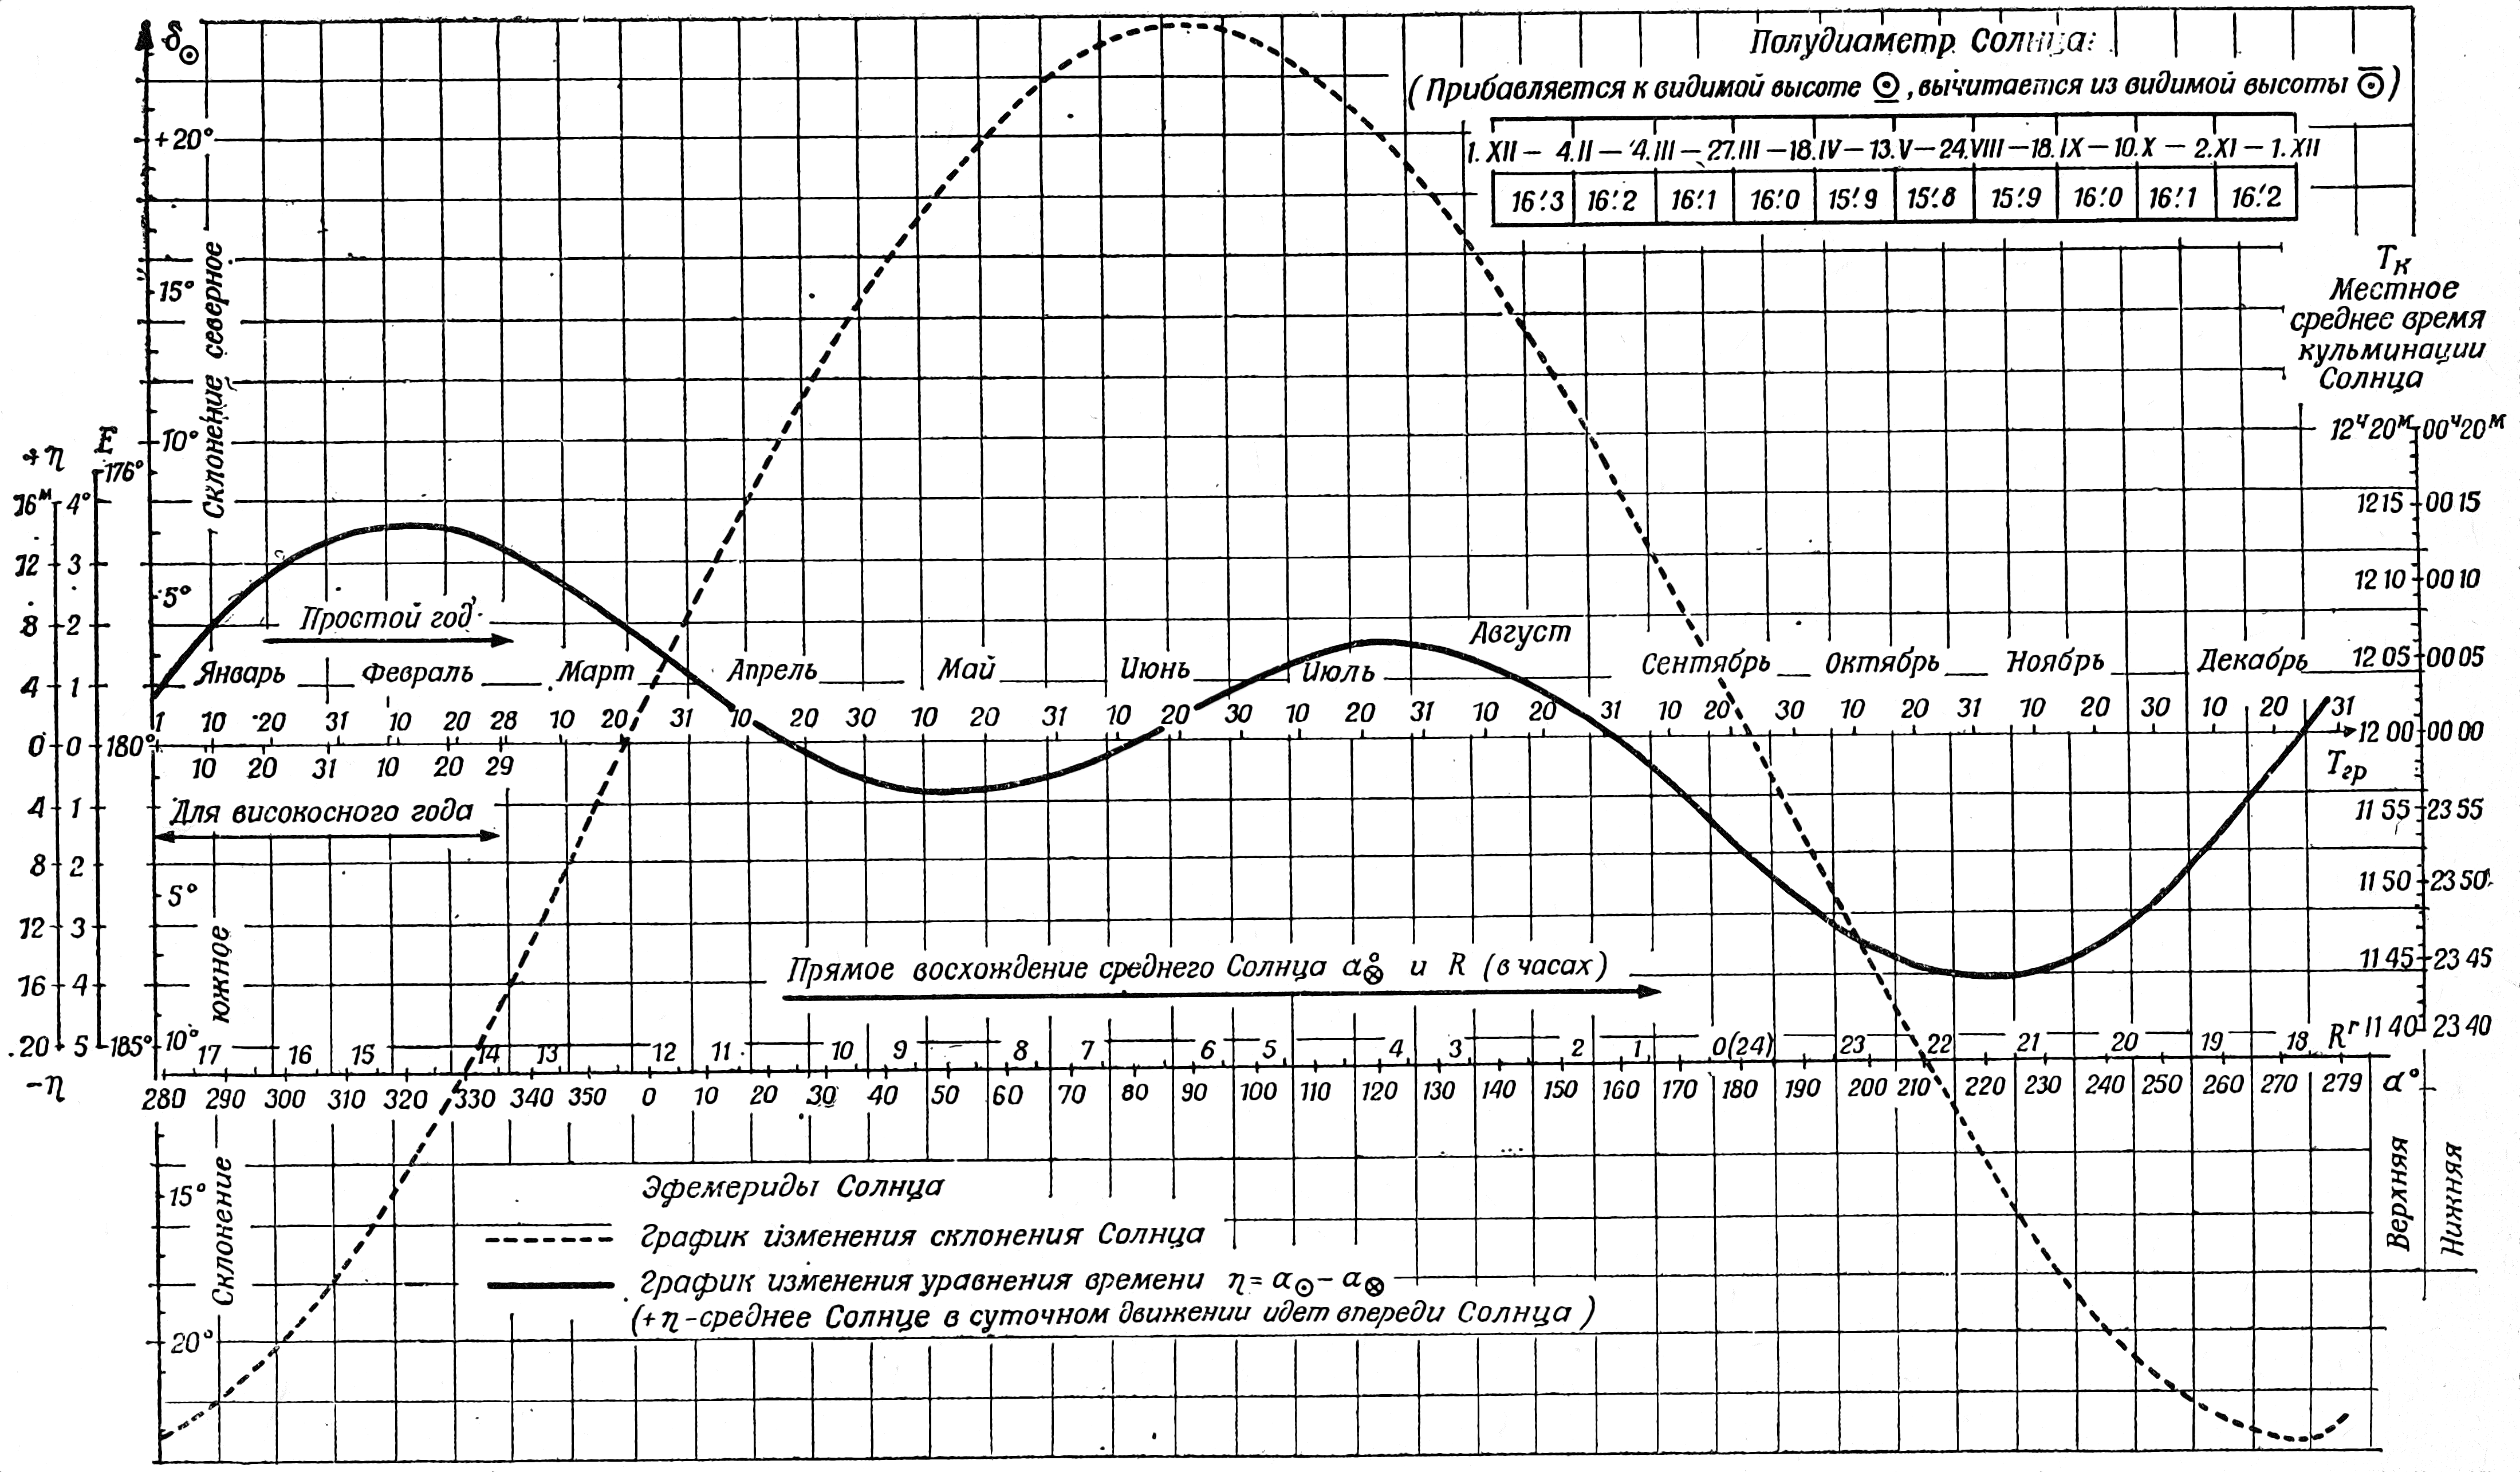
\includegraphics[width=\textheight]{0147P.png}
  \caption{Эфемериды Солнца}
  \label{fig:147}
\end{sidewaysfigure*}

\begin{multicols}{2}
  На графике (\rris{147}) по горизонтальной оси нанесена шкала для
  отсчёта календарных дат простого и високосного года, а также
  моментов всемирного времени \Tgr (выраженных в долях суток). Слева
  даны вертикальные шкалы для получения:
%
  \begin{itemize}
  \item уравнения времени $\eta$ (в градусной и часовой мере),
  \item вспомогательной величины $E$ для вычисления часового угла
    Солнца,
  \item склонения Солнца $\delta$.
  \end{itemize}
%
  Справа дана шкала для получения моментов наступления полудня $T_K$
  (верхняя кульминация) и полуночи по меридианному (местному) среднему
  времени.

  По нижней шкале получают прямое восхождение среднего солнца
  $\alpha^\otimes$ и вспомогательную величину $R$ (в часовой мере) для
  перехода от среднего времени $T$ к звёздному времени $t_V$ и
  обратно.

  Все необходимые величины выбираются путём непосредственной
  глазомерной интерполяции на шкалах графика с помощью
  циркуля-измерителя; их погрешность составляет около
  $0,2\gr = 1\tmin$. Полученные по графику эфемериды можно применять
  при расчётах освещённости горизонта, при работе со звёздной картой и
  звёздным глобусом, при определении направления движения яхты и
  поправки компаса по Солнцу (с точностью до 0,5\gr), при
  ориентировании по высоте Солнца (в тех случаях, когда она
  приближённо измерена самодельной астролябией).

  \begin{small}
    \textbf{Пример А.} 26 июля в момент $\Tgr = \hhmm{17}{36}$ вычислить
    часовой угол Солнца и его склонение. Долгота места яхты
    $\lambda = \grmmr{31}{50}{W}$.
    
    \textbf{Решение:}
    \begin{enumerate}
    \item Выражаем \Tgr в долях суток:
      $17,6\thr / 24\thr = 0,7~\text{сут.}$
    \item Входом по 26 июля $\Tgr = 0,7~\text{сут.}$ с точечной кривой
      графика получаем склонение Солнца $\delta = 19,4\gr$.
    \item Таким же входом по сплошной кривой получаем $E = 178,4\gr$.
    \item Вычисляем часовой угол Солнца:
    \end{enumerate}
  \end{small}
\end{multicols}

\begin{small}
  \begin{itemize}
  \item[1.] Всемирное время в градусной мере по прилож.\appnav{б}: $\Tgr = 264,0\gr$
  \item[2.] Вспомогательная величина $E$ (всегда прибавляется): $E = 178,4$
  \item[3.] Гринвичский часовой угол Солнца ($\ppp1 + \ppp2$): $\tGR = 442,4\gr W$
  \item[4.] Долгота места яхты $\lambda$ ($\Ost$ \--- плюс, $W$ \--- минус): $\lambda=31,8\gr$
  \item[5.] Местный часовой угол Солнца ($\ppp3 + \ppp4$): $\cidx{t}{м} = 410,6\gr W$
  \item[6.] Вычесть 360\gr, если $\cidx{t}{м} > 360\gr$: $\cidx{t}{м} = 50,6\gr W$
  \item[7.] Восточный часовой угол, если $\cidx{t}{м} > 180\gr$
  \end{itemize}
\end{small}

\begin{multicols}{2}
  \begin{small}
    \textbf{Пример Б.} 28 июля вычислить судовое время верхней кульминации Солнца (момент наступления полудня) в долготе \grmmr{150}{59}{\Ost}). Часы на яхте установлены по летнему времени Владивостока ($\mathNo_C = 11\Ost$).
    
    \textbf{Решение:} По календарной дате и сплошной кривой графика на шкале справа получаем:
  \end{small}
\end{multicols}

\begin{small}
  \begin{itemize}
  \item[1.] Меридианное время верхней кульминации: $T_K = \hhmm{12}{06}$
  \item[2.] Долгота места (восточную \--- отнять, западную \--- прибавить)
    в часовой мере по прилож.\appnav{б}: $\lambda = \hhmm{10}{04}$
  \item[3.] Всемирное время, 28 июля ($\ppp1 \pm \ppp2$): $\Tgr = \hhmm{2}{02}$
  \item[4.] Часовой пояс, принятый на яхте (восточный \--- плюс): $\mathNo_C = 11\Ost$
  \item[5.] Судовое время верхней кульминации ($\ppp3 \pm \ppp4$): $T_C = \hhmm{13}{02}$
  \end{itemize}
\end{small}

...раздел не окончен...

%%% Local Variables:
%%% mode: latex
%%% TeX-master: "yacht-captain"
%%% End:
